\documentclass{beamer}
\usepackage[english]{babel}
\usefonttheme{professionalfonts}
\usepackage{geometry}
\usepackage{amsmath}
\usepackage{amsthm}
\usepackage{graphicx}
\usepackage{caption}
\usepackage[utf8]{inputenc}


%%%%%%%% SUB-FIGURE PACKAGE
\usepackage{subcaption}

%%%%%%%% MULTI-COLUMNS PACKAGE
\usepackage{multicol}

%%%%%%%% PERSONAL COMMANDS
\usepackage{amssymb}

%%%% Important sets
\renewcommand{\O}{\mathbb{O}}
\newcommand{\N}{\mathbb{N}}
\newcommand{\Z}{{\mathbb{Z}}}
\newcommand{\Q}{{\mathbb{Q}}}
\newcommand{\R}{{\mathbb{R}}}

%%%% Usual operations
\newcommand{\pow}[2]{#1^{#2}}
\newcommand{\expp}[1]{e^{#1}}
\newcommand{\fst}{\mathrm{fst}}
\newcommand{\snd}{\mathrm{snd}}

%%%% Lambda Calculus
\newcommand{\dneq}{\,\, \# \,\,}
\newcommand{\prm}[1]{\pmb{\mathrm{#1}}}
\renewcommand{\S}{\prm{S}}
\newcommand{\I}{\prm{I}}
\newcommand{\K}{\prm{K}}
\newcommand{\ch}[1]{\ulcorner #1 \urcorner}

%%%% Ordinal Lambda Calculus
\newcommand{\ordAlph}{\Sigma_{\text{Ord}}}
\newcommand{\termOrd}{\text{Term}_\text{Ord}}
\newcommand{\fl}{\mathrm{fl}}
\newcommand{\sk}{\mathrm{sk}}

%% Superscript to the left
% https://latex.org/forum/viewtopic.php?t=455
\usepackage{tensor}
\newcommand{\app}[3]{\tensor*[^{#1}]{\left(#2, #3\right)}{}}

%%%% Make optional parameter
% https://bit.ly/3jVGRwQ
\usepackage{xparse}

%%%% Statistics
\NewDocumentCommand{\E}{o m}{
  \IfNoValueTF{#1}
  {\mathbb{E}\left[#2\right]}
  {\mathbb{E}^{#1}\left[ #2\right]}
}
\NewDocumentCommand{\V}{o m}{
  \IfNoValueTF{#1}
  {\mathrm{Var}\left[#2\right]}
  {\mathrm{Var}^{#1}\left[ #2\right]}
}
\RenewDocumentCommand{\P}{o o m}{
  \IfNoValueTF{#1}
  {\IfNoValueTF{#2}
    {\mathrm{P}\left(#3\right)}
    {\mathrm{P}^{#2}\left(#3\right)}}
  {\IfNoValueTF{#2}
    {\mathrm{P}_{#1}\left(#3\right)}
    {\mathrm{P}_{#1}^{#2} \left(#3\right)}}
}

%%%% Lambda Calculus
\NewDocumentCommand{\cx}{o}{
  \IfNoValueTF{#1}
  {\left[\quad\right]}
  {\left[\, #1 \,\right]}
}

%%%% Create absolute value function
% https://bit.ly/33Rkq6H
\usepackage{mathtools}
\DeclarePairedDelimiter\abs{\lvert}{\rvert}%
\DeclarePairedDelimiter\norm{\lVert}{\rVert}%
\makeatletter
\let\oldabs\abs
\def\abs{\@ifstar{\oldabs}{\oldabs*}}
%
\let\oldnorm\norm
\def\norm{\@ifstar{\oldnorm}{\oldnorm*}}
\makeatother

%%%%%%%% LOGIC TREES
\usepackage{prftree}

%%%%%%%% SPLIT EQUATIONS
% https://bit.ly/33P1OUM
\allowdisplaybreaks

%%%%%%%% FLOAT SPECIFIER
% https://bit.ly/30Wi4BC
\usepackage{float}

%%%%%%%% TO USE SHORT COMMANDS FOR VECTOR LINES
\usepackage{esvect}

%%%%%%%% ENUMERATE LABEL
% https://www.latex-tutorial.com/tutorials/lists/
\usepackage{enumitem}

%%%%%%%% DIFFERENT FONTS FOR MATH
\usepackage{mathrsfs}


%%%%%%%% HYPERREF PACKAGE
\hypersetup{colorlinks=true}
\hypersetup{citecolor=orange}
\hypersetup{urlcolor=orange}

%%%%%%%% DEFINITION AND THEOREM DEFINITIONS
\let\definition\relax
\theoremstyle{definition}
\newtheorem{definition}{Definition}[section]

\let\remark\relax
\theoremstyle{remark}
\newtheorem{remark}{Remark}

\theoremstyle{example}
\newtheorem{question}{Question}

%%%%%%%% BIB-LATEX STUFF
\usepackage[style=numeric,
            bibstyle=numeric,
            citestyle=numeric,
            hyperref=true,
            backend=biber]{biblatex}
\addbibresource{ref.bib} % Bibliography file

%%%%%%%% ICONS FOR CITES
% https://tex.stackexchange.com/questions/68080/beamer-bibliography-icon
\setbeamertemplate{bibliography item}{%
  \ifboolexpr{ test {\ifentrytype{book}} or test {\ifentrytype{mvbook}}
    or test {\ifentrytype{collection}} or test {\ifentrytype{mvcollection}}
    or test {\ifentrytype{reference}} or test {\ifentrytype{mvreference}} }
    {\setbeamertemplate{bibliography item}[book]}
    {\ifentrytype{online}
       {\setbeamertemplate{bibliography item}[online]}
       {\setbeamertemplate{bibliography item}[article]}}
  \usebeamertemplate{bibliography item}}

\defbibenvironment{bibliography}
  {\list{}
     {\settowidth{\labelwidth}{\usebeamertemplate{bibliography item}}
      \setlength{\leftmargin}{\labelwidth}
      \setlength{\labelsep}{\biblabelsep}
      \addtolength{\leftmargin}{\labelsep}
      \setlength{\itemsep}{\bibitemsep}
      \setlength{\parsep}{\bibparsep}}}
  {\endlist}
  {\item}

%%%%%%%% BRACKETS AROUND CITE
% https://bit.ly/3iSxP2u
\makeatletter

\newrobustcmd*{\parentexttrack}[1]{
  \begingroup
  \blx@blxinit
  \blx@setsfcodes
  \blx@bibopenparen#1\blx@bibcloseparen
  \endgroup}

\AtEveryCite{
  \let\parentext=\parentexttrack
  \let\bibopenparen=\bibopenbracket
  \let\bibcloseparen=\bibclosebracket}

\makeatother

%%%%%%%% THEME SLIDES
\usetheme{default}

%%%%%%%% BEAMER STUFF
\setbeamertemplate{footline}[frame number]
\setbeamertemplate{section in toc}[sections numbered]
\setbeamertemplate{subsection in toc}[subsections numbered]
\setbeamertemplate{navigation symbols}{}

% Not enumerate frame breaks
% https://bit.ly/34Rc6TG
\setbeamertemplate{frametitle continuation}[from second][]

%%%%%%%% FRAME TITLES AND SUBTITLES
% https://bit.ly/2FqgWP2
\newif\ifinsection
\newif\ifinsubsection

\let\oldsection\section
\renewcommand{\section}{
  \global\insectiontrue
  \global\insubsectionfalse
  \oldsection}
\let\oldsubsection\subsection
\renewcommand{\subsection}{
  \global\insubsectiontrue
  \oldsubsection}

\newcommand {\aframe}[1] {
  \begin{frame}
    \ifinsection\frametitle{\secname}\fi
    \ifinsubsection\framesubtitle{\subsecname}\fi
  #1
  \end{frame}
}

% Blue line after title
% https://bit.ly/33P6hXm
\setbeamertemplate{frametitle}{%
    \usebeamerfont{frametitle}\insertframetitle\strut%
    \vskip.0\baselineskip%
    \leaders\vrule width 0.85\paperwidth\vskip0.4pt%
    \vskip2pt%
    \usebeamerfont{framesubtitle}\insertframesubtitle
}

% Footnote without symbol
% https://tex.stackexchange.com/questions/30720/footnote-without-a-marker
\newcommand\blfootnote[1]{%
  \begingroup
  \renewcommand\thefootnote{}\footnote{#1}%
  \addtocounter{footnote}{-1}%
  \endgroup
}

%%%%%%%% CENTER OF SLIDE THANK YOU
\usepackage{tikz}

%%%%%%%% CODE RENDERING !!! UNCOMMENT IF NEEDED !!!
% Compile with flag -shell-escape
%\usepackage{minted}


%%%%%%%% START DOCUMENT
\title{Evaluation of Robust Covariance Estimation for Object Localization}

\author{Juan Sebasti\'an C\'ardenas-Rodríguez \\
  Andr\'es Felipe Tamayo-Arango \\
  David Plazas Escudero \\
  \scalebox{0.7}{Mathematical Engineering, Universidad EAFIT}}

\begin{document}

% Plain so is not numbered
\begin{frame}[plain]
  \titlepage
\end{frame}

%%%%%%%%%% SLIDES %%%%%%%%%%%%%%%
\section{Introduction}
\subsection{Motivation}
\aframe{
  \begin{itemize}
    \item ``Anything from identifying a location to identifying and registering
          components of a particular object class at various levels of
          detail''\parencite{amit20022d}.
    \item Computer vision: how computers can understand digital images and
          videos, similar to how human visual system
          works\parencite{ballard1982computer,huang1996computer,
          amit20022d,szeliski2010computer}.
  \end{itemize}
  \begin{figure}[H]
    \centering 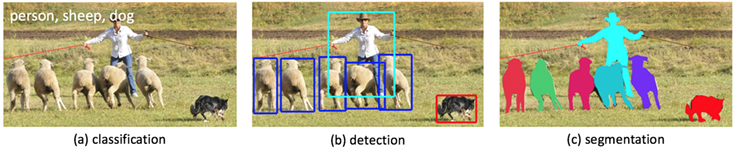
\includegraphics[width=\linewidth]{figs/objs.jpg}
    \caption{Computer vision tasks\footnote{taken from
        \href{https://bit.ly/2JTXLid}{this article}.}}
    \label{fig:tasks}
  \end{figure}
}

\subsection{Scope}
\aframe{ \textbf{Objectives}
  \begin{enumerate}
    \item Make fast implementations for the robust covariances, specially
          Kendall, Spearman and the Comedian estimation. \pause
    \item Evaluate the metric's and covariance matrix efficiency in the
          algorithm.
  \end{enumerate} \pause \vspace{0.5cm}

  \textbf{Limitations}
  \begin{enumerate}
    \item We're undergraduate students, i.e. we're currently seeing
          \textbf{five} other subjects simultaneously. \pause
    \item We do not have access to cloud services. \pause
    \item We only participated in the Algebra in Data Science course, not the
          other two subjects needed for the complete project.
  \end{enumerate}
}
\subsection{Justification}
\aframe{ One of the main applications of the methodology used in this work is in
  Object Tracking, which is an immediate consequence of localization.\pause

  The works of Porikli, Tuzel \& Meer\parencite{porikli2006covariance} and Wu et
  al.\parencite{wu2012real} show outstanding results for object tracking, using
  real-time model update.
  \begin{itemize}
    \item\parencite{porikli2006covariance} takes the advantage of the Lie group
          structure of the covariance matrices and updates the average
          covariance through time with Lie algebra.
    \item\parencite{wu2012real} uses two stages at each frame: a Maximum A
          Posteriori propagation and a novel Incremental Covariance Tensor
          Learning online.
\end{itemize}
}

\aframe{
  \begin{itemize}
    \item Another important application is in face recognition: Pang, Yuang \&
          Li\parencite{pang2008gabor} used the original Region Covariance method
          for face recognition but adding Gabor Wavelet features to improve the
          performance.\pause
    \item Finally, an application in license plate detection has been developed
          as well by Porliki \& Kocak\cite{porikli2006robust}. The different
          covariance region descriptors are fed (flattened) into a multi-layer
          perceptron that determines if the region is or not a license plate.
          This results in a faster algorithm than calculating dissimilarities.
    \end{itemize}
}

\section{Methodology}
\subsection{CRISP-DM}
\aframe{
  \begin{figure}[H]
    \centering 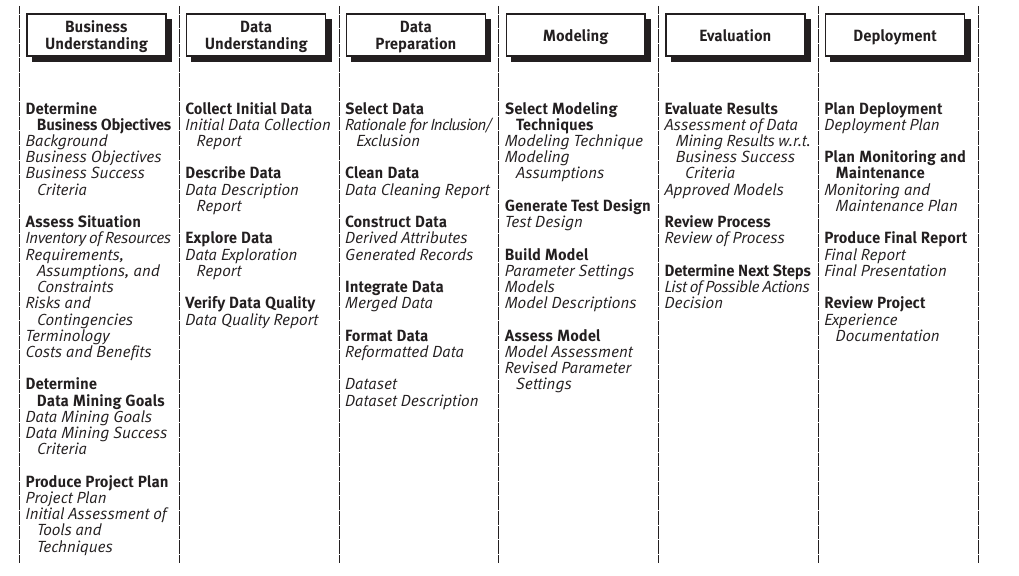
\includegraphics[width = \linewidth]{figs/crisp-dm.png}
    \caption{CRISP-DM Methodology (taken from\cite{Chapman2000CRISPDM1S}).}
  \end{figure}
}

\subsection{Region Covariance}
\aframe{ For an image of width $W$ and height $H$, let
  $\mathcal{W}=\{1,\ldots,W\}$ and $\mathcal{H}=\{1,\ldots,H\}$. The image is
  then mapped into a feature space for each pixel
  \[
    F:\mathcal{W}\times\mathcal{H}\rightarrow\mathbb{R}^{d}
  \]
  yielding a tensor $\mathcal{A} \subset \R^{W \times H \times d}$.
  \begin{figure}[H]
    \centering 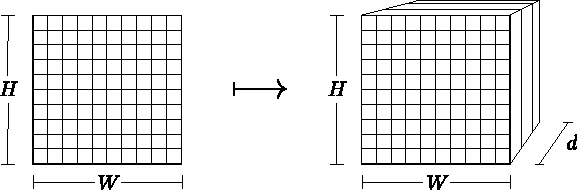
\includegraphics[width =
    0.9\linewidth]{figs/feature_extraction.pdf}
    \caption{Feature extraction.}
  \end{figure}
}

\aframe{ Let $W'$ and $H'$ the width and height of region $R\subset\mathcal{A}$.
  The covariance matrix of $R$ is estimated by flattening the region into a
  $(W'\cdot H')\times d$ data matrix, yielding
  $\mathbf{C}_R \in \R^{d \times d}$.
  \begin{figure}[H]
    \centering

    \only<1>{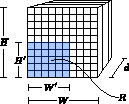
\includegraphics[width = 0.55\linewidth]{figs/region1.pdf}}
    \only<2>{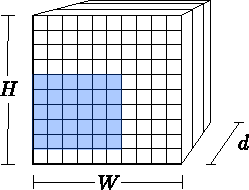
\includegraphics[width = 0.5\linewidth]{figs/region2.pdf}}
    \only<3>{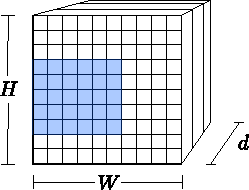
\includegraphics[width = 0.5\linewidth]{figs/region3.pdf}}
    \only<4>{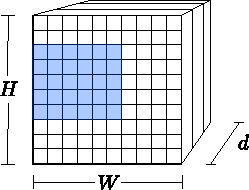
\includegraphics[width = 0.5\linewidth]{figs/region4.pdf}}
    \only<5>{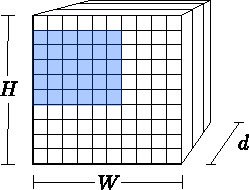
\includegraphics[width = 0.5\linewidth]{figs/region5.pdf}}
    \only<6>{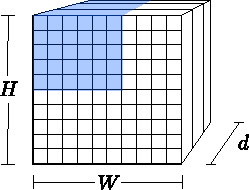
\includegraphics[width = 0.5\linewidth]{figs/region6.pdf}}
    \only<7>{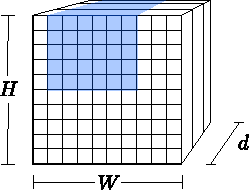
\includegraphics[width = 0.5\linewidth]{figs/region7.pdf}}
    \only<8>{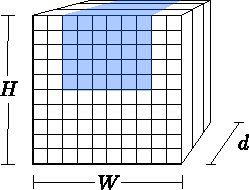
\includegraphics[width = 0.5\linewidth]{figs/region8.pdf}}
    \only<9>{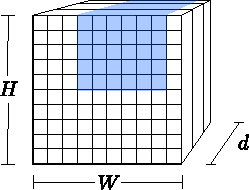
\includegraphics[width = 0.5\linewidth]{figs/region9.pdf}}
    \only<10>{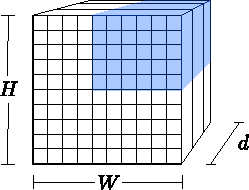
\includegraphics[width = 0.5\linewidth]{figs/region10.pdf}}
    \caption{Feature region.}
  \end{figure}
}

\aframe{ The methodology for object localization using region covariance
  \parencite{tuzel2006} will be now presented:

  \begin{overlayarea}{\textwidth}{0.7\textheight}
    \begin{enumerate}
            \only<1>{
      \item Estimate the covariance matrix of the target input object $T$.
      \item Search all possible regions $R$ in the target image for covariances
            with low dissimilarity $\rho(\mathbf{C}_R,\mathbf{C}_T)$, using
            different scales. The best 1000 locations are saved.

      \item Each of the 1000 regions is subdivided as follows:
            \begin{figure}[H]
              \centering 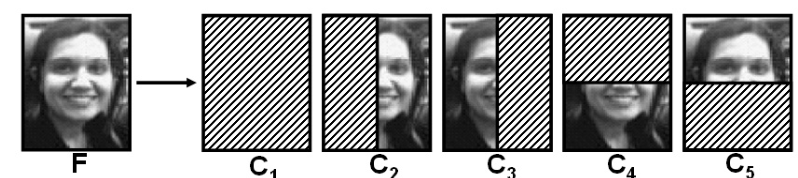
\includegraphics[scale=.4]{figs/regions.png}
              \caption{Region subdivision, image taken
                from\parencite{tuzel2006}.}
            \end{figure}
            } \only<2>{ \setcounter{enumi}{3}
      \item The region with minimum dissimilarity, calculated as follows, is
            selected as the matching region
            \begin{equation*}
              \lambda(R, T)=\min _{j}\left[\sum_{i=1}^{5} \rho\left(
                  \mathbf{C}_{i}^{R}, \mathbf{C}_{i}^{T}\right)-\rho\left(
                  \mathbf{C}_{j}^{R}, \mathbf{C}_{j}^{T}\right)\right]
            \end{equation*}
            }
    \end{enumerate}
  \end{overlayarea}}

\aframe{ The selected $d=9$ features are
  \begin{align*}
    F(x, y)=&\left[x,\, y,\, R(x, y),\, G(x, y),\, B(x, y),\right.\\
            &\left.\left|\frac{\partial I(x, y)}{\partial x}
              \right|,\,\left|\frac{\partial I(x, y)}
              {\partial y}\right|,\,\left|\frac{\partial^{2} I(x, y)}
              {\partial x^{2}}\right|,\,\left|\frac{\partial^{2} I(x, y)}
              {\partial y^{2}}\right|\right]^{T}
  \end{align*}
  yielding a covariance matrix $\mathbf{C}_R\in\mathbb{R}^{9\times 9}$ for each
  region $R$.
  \begin{itemize}
    \item RGB color scheme.
    \item Derivatives estimated through Sobel filters:
          \begin{itemize}
            \item Edge detection.
            \item Spatial relations.
            \item Kernel convolution.
          \end{itemize}
  \end{itemize}
}

\subsection{Metrics}
\aframe{ Two metrics of dissimilarity are used:
  \begin{enumerate}
    \item The one induced by the Frobenius norm:
          \[
            \rho(\mathbf{C}_1, \mathbf{C}_2)
            =\norm{\mathbf{C}_1-\mathbf{C}_2}_F=\sqrt{\mathrm{tr}(\mathbf{C}_1
              -\mathbf{C}_2)^T(\mathbf{C}_1-\mathbf{C}_2)}
          \]\pause
    \item The one proposed by F\"orstner \&
          Moonen\parencite{forstner2003metric}:
          \begin{equation}
            \rho\left(\mathbf{C}_{1}, \mathbf{C}_{2}\right)=\sqrt{
              \sum_{i=1}^{n} \ln ^{2} \lambda_{i}\left(\mathbf{C}_{1}
                , \mathbf{C}_{2}\right)}
          \end{equation}
          where
          $\left\{\lambda_{i}\left(\mathbf{C}_{1}, \mathbf{C}_{2}\right)\right\}_{i=1}^n$
          are the generalized eigenvalues of $\mathbf{C}_{1}$ and
          $\mathbf{C}_{2},$ computed from
          \[
            \lambda_{i} \mathbf{C}_{1} \mathbf{x}_{i}-\mathbf{C}_{2}
            \mathbf{x}_{i}=0, \quad i=1 \ldots d
          \]
          and $\mathbf{x}_{i} \neq 0$ are the generalized eigenvectors.
  \end{enumerate}
}

\subsection{Covariance Estimation}
\aframe{ Five different covariance matrix estimators are used:
  \begin{enumerate}
    \item Maximum Likelihood Estimation.
    \item Comedian\parencite{falk1997mad}.
    \item Spearman\parencite{spearman1961general}.
    \item Kendall\parencite{kendall1938new}.
    \item Ledoit and Wolf\parencite{ledoit2004honey}.
  \end{enumerate} \pause
  %
  \begin{table}[]
    \centering
    \begin{tabular}{cccc}
      \hline
      & Spearman      & Kendall       & Comedian      \\
      Na\"ive (s)  & 1.44          & 162.13        & 369.78        \\
      Ours (s)   & \textbf{0.30} & \textbf{4.11} & \textbf{3.66} \\
      Na\"ive (MB) & \textbf{109}  & \textbf{108}  & \textbf{104}  \\
      Ours (MB)  & 115           & 1977          & 2020    \\     \hline
    \end{tabular}
    \caption{Tests with random matrix in $\R^{1000\times500}$.}
  \end{table}
}

\subsection{Noise Addition}
\aframe{The algorithm will be tested using some \textit{damaged} inputs by
  adding impulse noise to the input. This was added using \texttt{ImageMagick
    7.0.10}.
  \begin{figure}
    \centering
    \begin{subfigure}[b]{0.45\textwidth}
      \centering 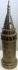
\includegraphics[height=0.55\textheight]{figs/input1.jpg}
      \caption{Input without noise.}
    \end{subfigure}
    %
    \begin{subfigure}[b]{0.45\textwidth}
      \centering
      
\includegraphics[height=0.55\textheight]{figs/input-impulse.jpg}
      \caption{Input with impulse noise.}
    \end{subfigure}
  \end{figure}
}

\section{Results}
\subsection{Image Results with Kendall Matrix}
\aframe{
  \begin{figure}
    \centering
    \begin{subfigure}[b]{0.32\textwidth}
      \centering 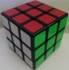
\includegraphics[width=\textwidth]{figs/input2.jpg}
      \caption{Input.}
    \end{subfigure}
    \begin{subfigure}[b]{0.32\textwidth}
      \centering 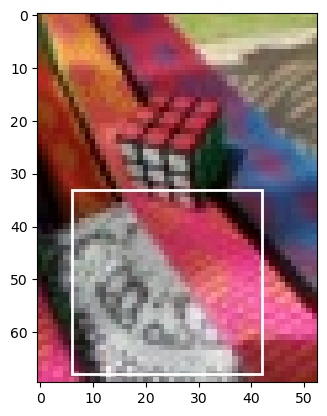
\includegraphics[width=\textwidth]{figs/0-3-0-test_case4.jpg}
      \caption{With noise.}
    \end{subfigure}
    \begin{subfigure}[b]{0.32\textwidth}
      \centering 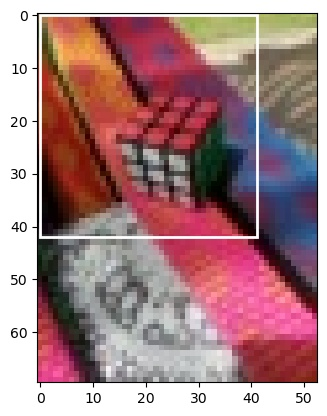
\includegraphics[width=\textwidth]{figs/1-3-0-test_case4.jpg}
      \caption{Without noise.}
    \end{subfigure}
    \caption{Tests for Rubik's cube with authors' metric.}
  \end{figure}
}

\aframe{
  \begin{figure}
    \centering
    \begin{subfigure}[b]{0.32\textwidth}
      \centering 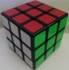
\includegraphics[width=\textwidth]{figs/input2.jpg}
      \caption{Input.}
    \end{subfigure}
    \begin{subfigure}[b]{0.32\textwidth}
      \centering 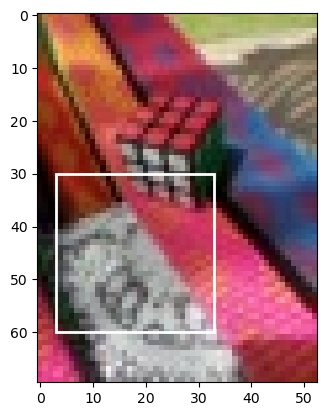
\includegraphics[width=\textwidth]{figs/0-3-1-test_case4.jpg}
      \caption{With noise.}
    \end{subfigure}
    \begin{subfigure}[b]{0.32\textwidth}
      \centering 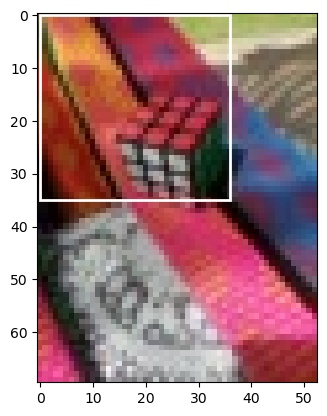
\includegraphics[width=\textwidth]{figs/1-3-1-test_case4.jpg}
      \caption{Without noise.}
    \end{subfigure}
    \caption{Tests for Rubik's cube with Frobenius metric.}
  \end{figure}
}

\aframe{
  \begin{figure}
    \centering
    \begin{subfigure}[b]{0.32\textwidth}
      \centering 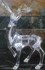
\includegraphics[width=\textwidth]{figs/input3.jpg}
      \caption{Input.}
    \end{subfigure}
    \begin{subfigure}[b]{0.32\textwidth}
      \centering 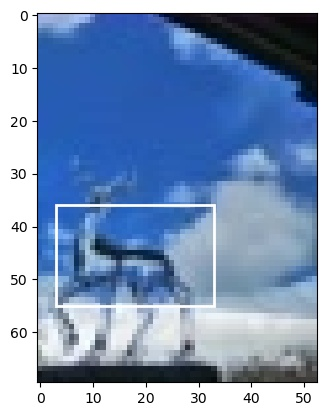
\includegraphics[width=\textwidth]{figs/0-3-0-test_case3.jpg}
      \caption{With noise.}
    \end{subfigure}
    \begin{subfigure}[b]{0.32\textwidth}
      \centering 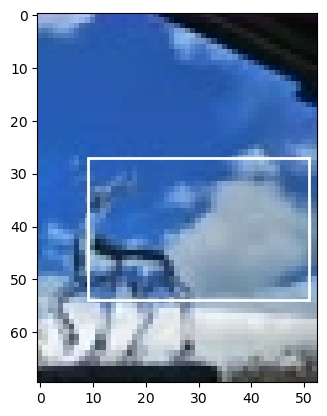
\includegraphics[width=\textwidth]{figs/1-3-0-test_case3.jpg}
      \caption{Without noise.}
    \end{subfigure}
    \caption{Tests for glass deer with authors' metric.}
\end{figure}
}

\aframe{ \onslide<2->{Using the Kendall matrix makes the algorithm the slowest.}
  \onslide<1->{\begin{figure} \centering
      \begin{subfigure}[b]{0.32\textwidth}
        \centering 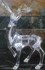
\includegraphics[width=0.9\textwidth]{figs/input3.jpg}
        \caption{Input.}
      \end{subfigure}
      \begin{subfigure}[b]{0.32\textwidth}
        \centering 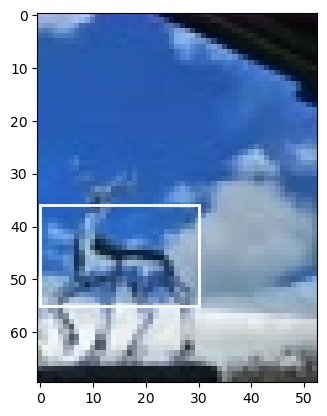
\includegraphics[width=\textwidth]{figs/0-3-1-test_case3.jpg}
        \caption{With noise.}
      \end{subfigure}
      \begin{subfigure}[b]{0.32\textwidth}
        \centering 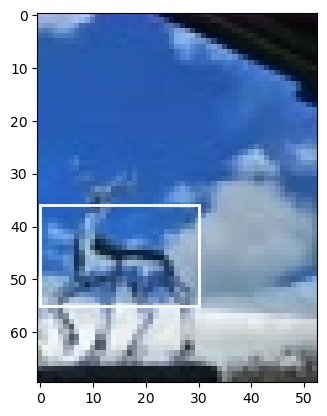
\includegraphics[width=\textwidth]{figs/1-3-1-test_case3.jpg}
        \caption{Without noise.}
      \end{subfigure}
      \caption{Tests for glass deer with Frobenius metric.}
\end{figure}}
}

\subsection{Image Results with LW}
\aframe{Another alternative with less precision is using LW, that yields a much
  faster algorithm. \pause
  \begin{figure}
    \centering
    \begin{subfigure}[b]{0.32\textwidth}
      \centering 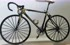
\includegraphics[width=\textwidth]{figs/input4.jpg}
      \caption{Input.}
    \end{subfigure}
    \begin{subfigure}[b]{0.32\textwidth}
      \centering 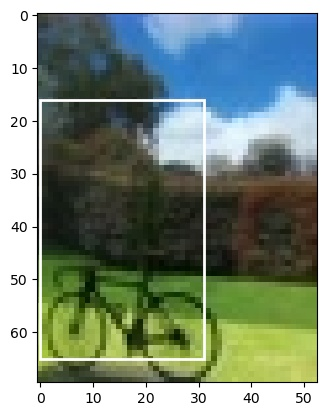
\includegraphics[width=\textwidth]{figs/0-4-0-test_case1.jpg}
      \caption{Authors' metric.}
    \end{subfigure}
    \begin{subfigure}[b]{0.32\textwidth}
      \centering 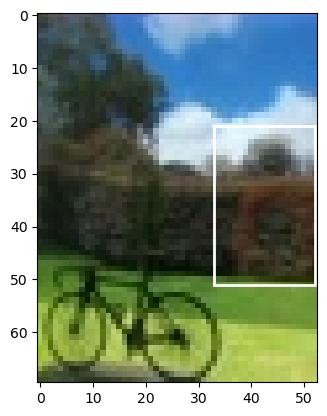
\includegraphics[width=\textwidth]{figs/0-4-1-test_case1.jpg}
      \caption{Frobenius metric.}
    \end{subfigure}
    \caption{Tests for bike with noise.}
\end{figure}
}

\subsection{Metrics}
\aframe{ The metrics were compared by setting a scatter plot of the distances to
  the real covariance matrix, using the Frobenius and the authors' dissimilarity
  measures:
  \begin{figure}[H]
    \centering 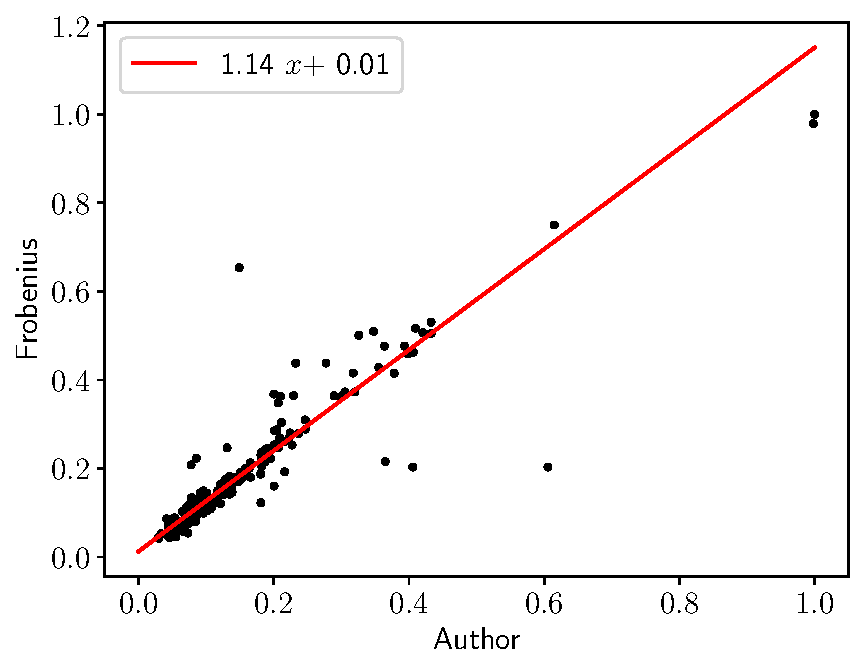
\includegraphics[width=0.5\linewidth]{figs/linear.pdf}
    \caption{Linear regression comparing metrics.}
  \end{figure}
}

\subsection{Covariance Matrices}
\aframe{
  \begin{figure}
    \centering 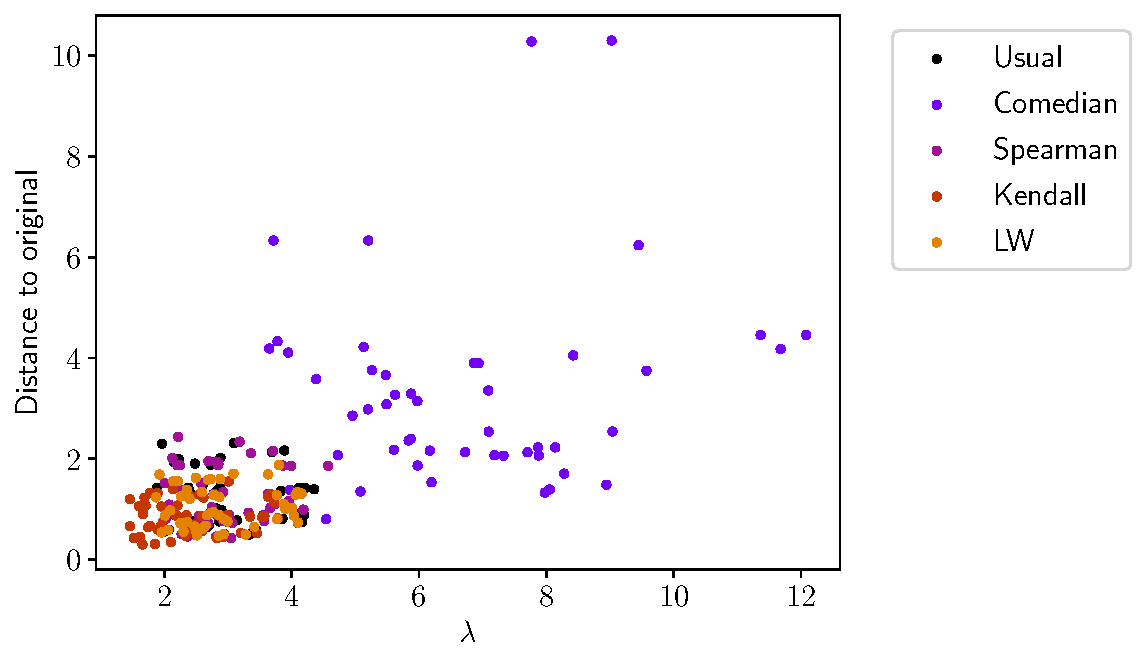
\includegraphics[width=0.9\textwidth]{figs/author-scatter.pdf}
    \caption{Pareto boundaries for covariance matrices (authors' metric).}
  \end{figure}
}

\aframe{
  \begin{figure}
    \centering 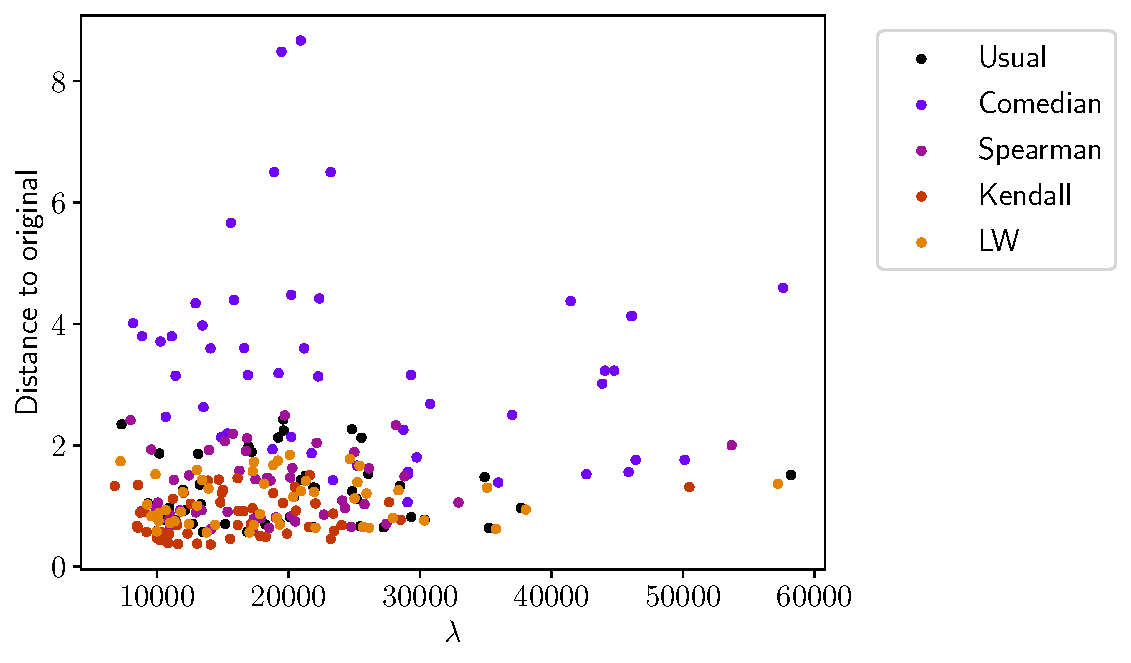
\includegraphics[width=0.9\textwidth]{figs/fro-scatter.pdf}
    \caption{Pareto boundaries for covariance matrices (Frobenius metric).}
  \end{figure}
}

\subsection{Noise}
\aframe{
  \begin{figure}
    \centering 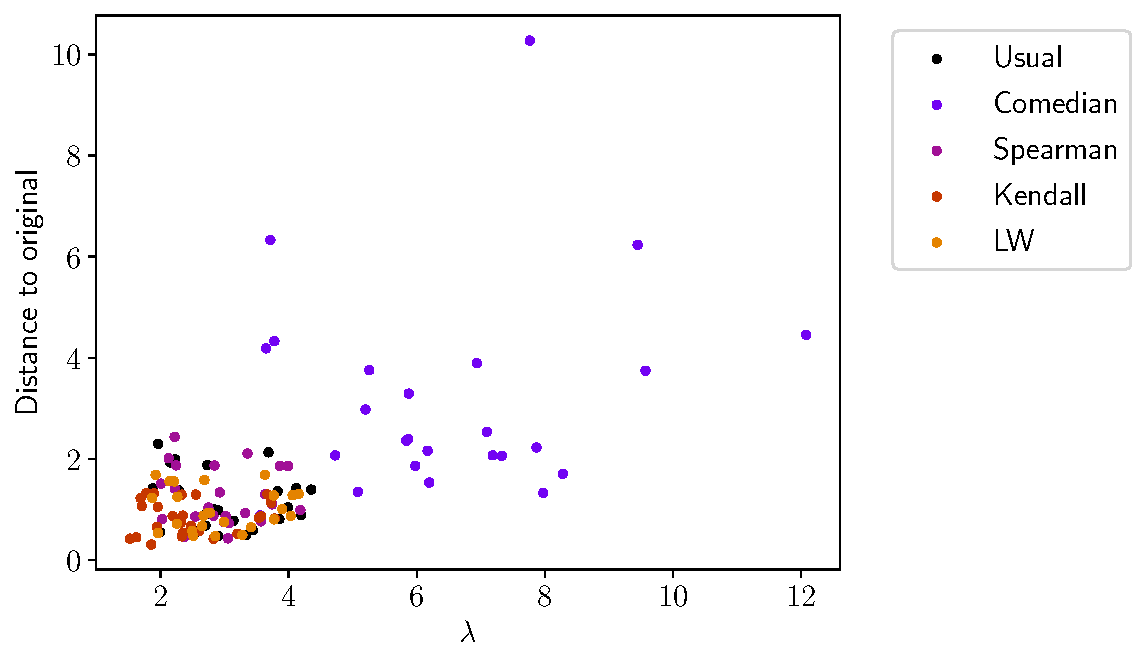
\includegraphics[width=0.9\textwidth]{figs/noise-scatter.pdf}
    \caption{Pareto boundaries for inputs with noise.}
  \end{figure}
}

\section{Concluding Remarks}
\aframe{
  \begin{itemize}
    \item Faster implementations for the robust covariance matrices were
          successfully achieved.\pause
    \item The two dissimilarity functions and the different covariance matrices
          were successfully evaluated for in different scenarios.\pause
    \item The overall best covariance matrix for object detection is the one
          based on Kendall's tau coefficient, although, it is the slowest. The
          Ledoit and Wolf estimation also gives good results with a faster
          execution time.\pause
    \item As for future work, the integral image data
          structure\parencite{porikli2005integral} could be used to accelerate
          the exploration of the regions on the image.
  \end{itemize}
}

%%%%%%%%%%%%%%%%%%%%%%%%%%%%%%%%%
\begin{frame}[allowframebreaks]{References}
  \printbibliography
\end{frame}

\begin{frame}
  \begin{tikzpicture}[overlay, remember picture]
    \node[anchor=center] at (current page.center) { \Huge{\emph{Thank you!}}};
  \end{tikzpicture}
  \begin{minipage}[t][.8\textheight]{\textwidth}
    \vfill
    \begin{center}
      \begin{multicols}{3}
        \scalebox{0.7}{Juan S. C\'ardenas-Rodríguez} \\
        \scalebox{0.7}{jscardenar@eafit.edu.co} \\
        \columnbreak
        \scalebox{0.7}{David Plazas-Escudero} \\
        \scalebox{0.7}{dplazas@eafit.edu.co} \\
        \columnbreak
        \scalebox{0.7}{Andrés F. Tamayo-Arango} \\
        \scalebox{0.7}{aftamayoa@eafit.edu.co}
      \end{multicols}
    \end{center}
  \end{minipage}
\end{frame}

\end{document}
